\subsubsection{}
The value of the initial position has been proved to be a draw\footnote{Ralph GASSER, \textit{Solving Nine Men's Morris}}. Therefore, if the time-per-move provided is long enough and if both players play with the same heuristic and manage to reach a depth of 3-4 in each turn search, then tey do not allow the rival to create a mill and the game will eventually end in a tie. This can explain the 20 sec result.

For a short time-per-move provided, both the players cannot get deep in the search and most of the time they stay in the same one (1.1 sec case). We assume that our heuristic makes it an easier game for Black (player 2), in the sense that it is better defend and stop the rival than attack and take initiative.

For medium-range time per move (5 sec and 10 sec) Alpha-beta is winning. It is enough time for alpha-beta to get more depth than the minimax player and winning the game.

The results are shown in Fig. \ref{fig:partF_1}.
\begin{figure}[h]
    \centering
    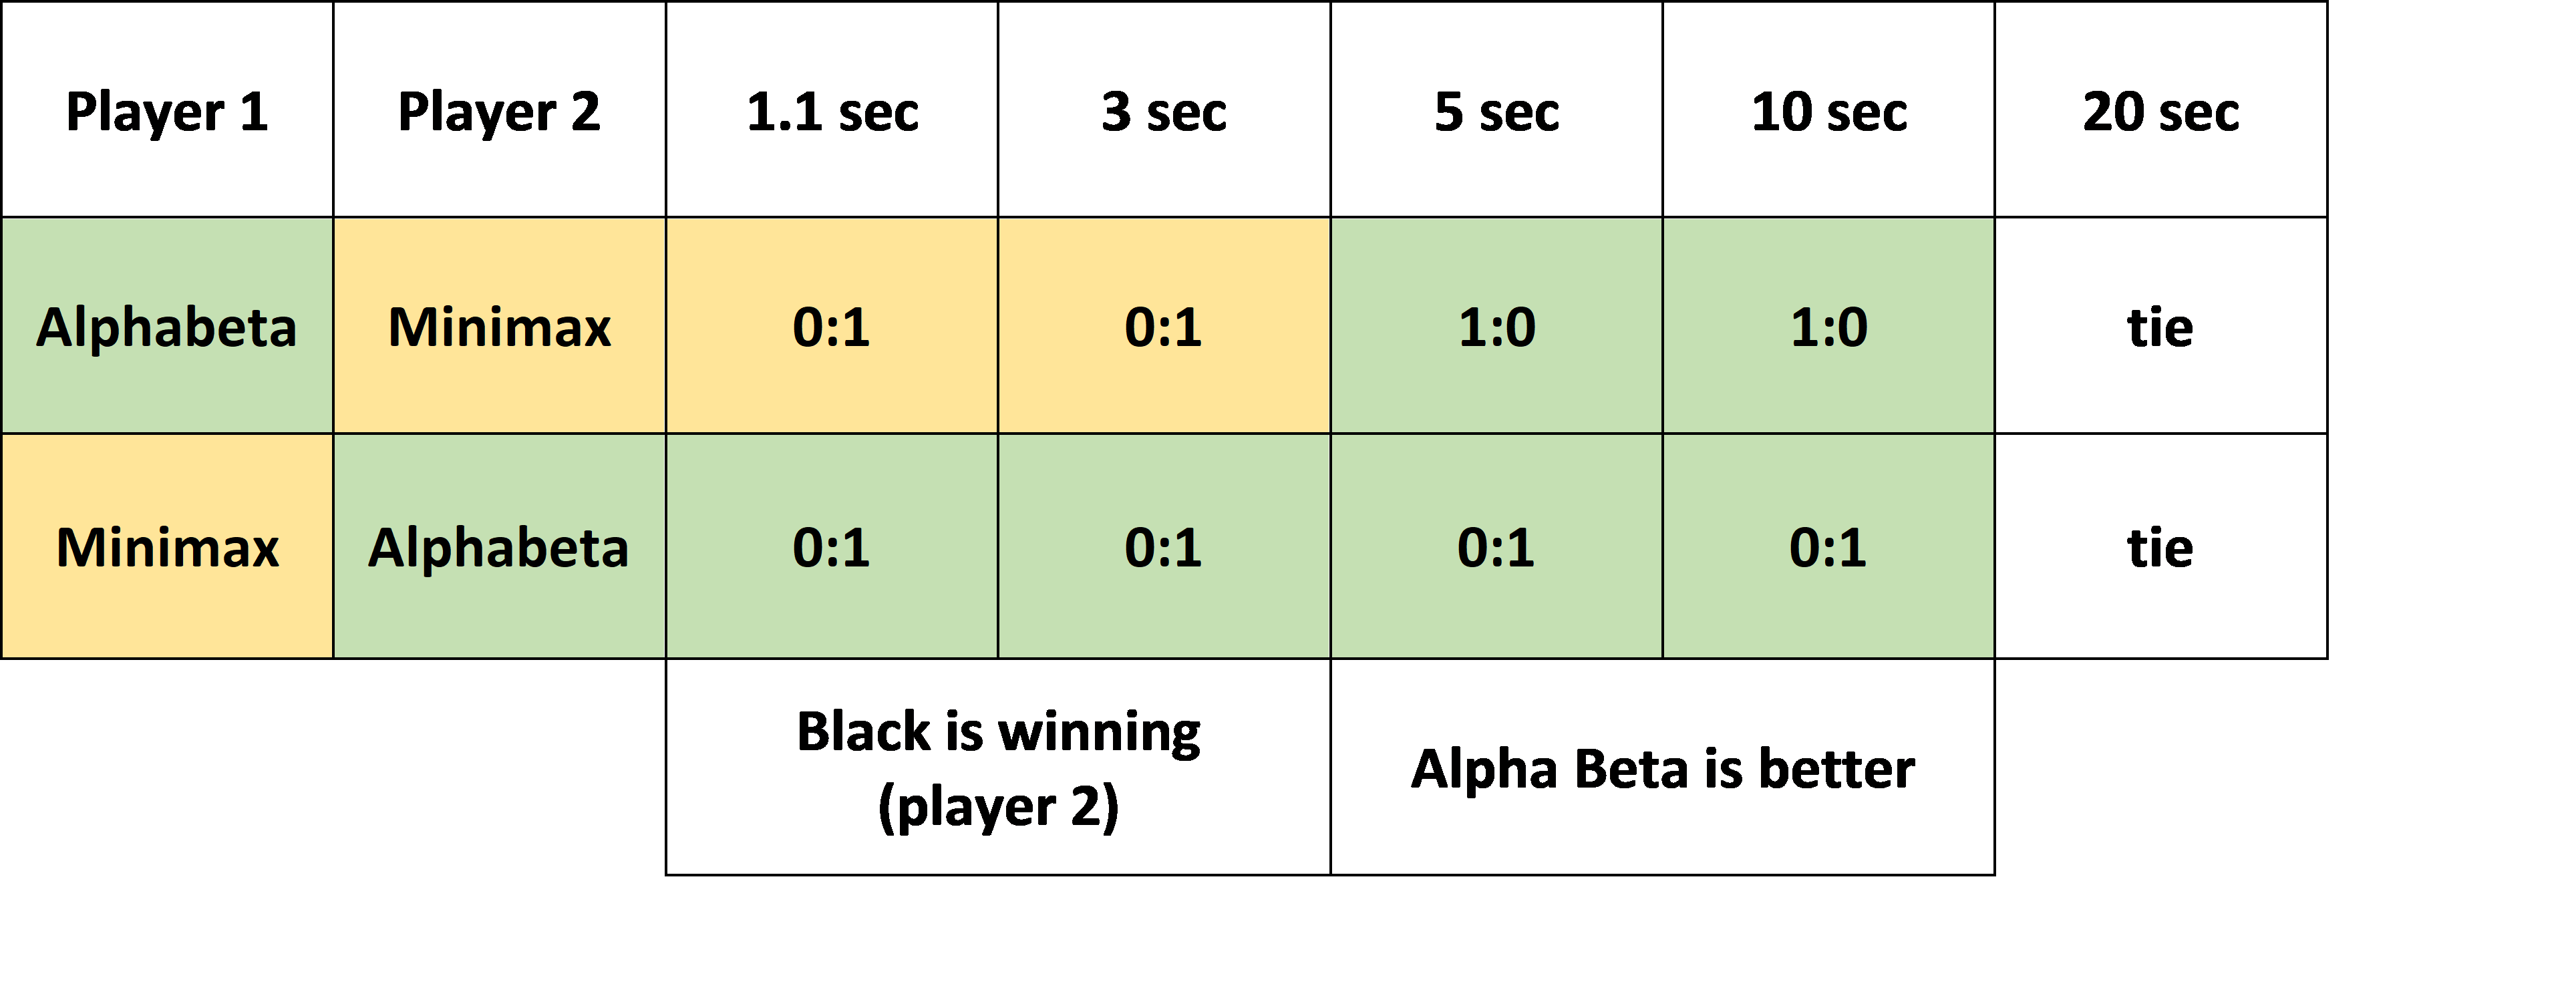
\includegraphics[width=1\linewidth]{partF_1}
    \caption{Rsults of the experiments for different time-per-move limits.}
    \label{fig:partF_1}
\end{figure}



\subsubsection{}
\textbf{Results}
For $depth=3$ we won with our Heavy Player in all the depth differences. For $depth=$ all the games ended in a tie (Program paused).

\textbf{Discussion}
Depth 3 experiments are understandable - the light heuristic was not informed enough - it does not have parameters such as – the difference between number of blocked soldiers, double mills, - piece configurations. So even the light player get higher depth, he is so far away from the endgame/terminal positions and without good evaluation of the positions he is loosing to the more informed player.

Depth 2 is strange, especially after the discussion of the depth 3 results. In all the games we stopped the game cause it’s just gets in a loop where no one want to loose and no one going for a new mill. The more informed player is usually in a better position but he can’t win. The explanation is that for winning he need to move one of the soldiers in a mill to construct a mill in the next move. But our heavy player is a two depth player so it only calculate his move and the rival’s one, so he can’t reach the mill (which constructed only in $depth=3$).

The conclusion is that $depth=2$ is not enough for our players and heuristic.

Te plots of the results concerning this are shown in Fig. \ref{fig:partF_collettivo}.
\begin{figure}[h]
    \centering
    \begin{subfigure}[b]{0.5\linewidth}
        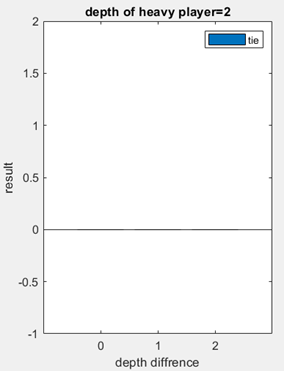
\includegraphics[width=\linewidth]{partF_2}
        \caption{$depth=2$}
        \label{}
    \end{subfigure}

    \begin{subfigure}[b]{0.5\linewidth}
        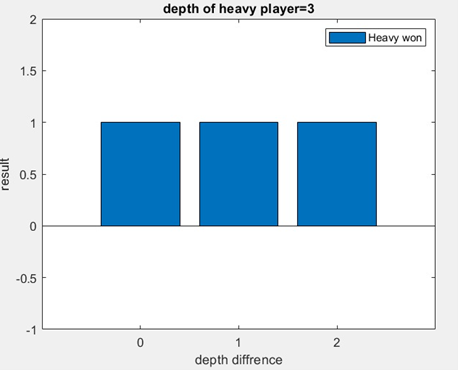
\includegraphics[width=\linewidth]{partF_3}
        \caption{$depth=3$}
        \label{}
    \end{subfigure}
    \caption{Heavy player for $depth=2,3$.}
    \label{fig:partF_collettivo}
\end{figure}